%%%%%%%%%%%%%%%%%%%%%%%%%%%%% TCC %%%%%%%%%%%%%%%%%%%%%%%%%%%%%%%%
%
% Template para TCC da Universidade Federal da Paraíba
%
% Autores: Elaine Soares elaineanita1@gmail.com
%          Rafael Brayner rafabrayner92@gmail.com
%          Roberto Júnior contato@robertojunior.net
%
% ShareLaTeX porting: Gustavo Sobral ghsobral@gmail.com
% 
% Revisão: Eudisley Anjos eudisley@ci.ufpb.br
%
% Sinta-se livre para melhorar e contribuir com esse projeto. 
%
%%%%%%%%%%%%%%%%%%%%%%%%%%%%%%%%%%%%%%%%%%%%%%%%%%%%%%%%%%%%%%%%%%%

\documentclass{tcc}

\begin{document}
\pagestyle{empty} %retira numeração da página
%Dados do TCC%
\author{Willian Marques Freire}
\title{IoT e integração com Micro-serviços}
\newcommand{\subtitulo}{Subtítulo}
\newcommand{\nomedocurso}{Ciência da Computação}
\newcommand{\titulobar}{Ciência da Computação}
\newcommand{\orientador}{Munif Gebara Júnior}
\newcommand{\profa}{Nome do Professor A}
\newcommand{\profb}{Nome do Professor B}
\newcommand{\profc}{Nome do Professor C}
\newcommand{\insta}{Instituicao do Professor A}
\newcommand{\instb}{Instituicao do Professor B}
\newcommand{\instc}{Instituicao do Professor C}
\newcommand{\coordenador}{Nome do Coordenador}
\newcommand{\departamento}{Nome do Departamento}

\begin{center}
\LARGE{\bf
Fundação Faculdade de Filosofia, Ciências e Letras de Mandaguari
}\\
\Large{\bf
    Curso de Ciência da Computação
}
\end{center}
\begin{figure}[H]
\vspace*{3cm}
\centering

\includegraphics[width=100mm]{imagens/logo2.jpg}
\vspace*{3cm}
\end{figure}


\begin{center}
\LARGE{\bf \thetitle:}\\
\Large{\bf \subtitulo}\\
\end{center}

\vspace{1em}

\vfill

\vspace{2in}

\begin{center}
\bf\theauthor
\vspace*{2cm}
\end{center}

\begin{center}
Mandaguari, \the\year
\end{center}
\afterpage{\blankpage \addtocounter{page}{1}} %addtocounter incrementa numero da pagina ja que blankpage nao entra no contador%

\newpage
\begin{center}
\theauthor
\end{center}
\vspace{3in}
\begin{center}
\LARGE{\thetitle}\\
\end{center}

\vspace{2in}

\begin{flushright}
Monografia apresentada ao curso \nomedocurso \\ do Centro de Informática, da Universidade Federal da Paraíba, \\ como requisito para a obtenção do grau de Bacharel em \titulobar
\\
\vspace{0.2in}

Orientador: \orientador


\end{flushright}

\vfill
\begin{center}
\MONTH de \the\year
\end{center}

\newpage

$ $
\vfill


\begin{flushright}
\fbox{\parbox[t][15em][c]{0.90\linewidth}{
\vspace{0.5in}

$\qquad$ Ficha catalográfica: elaborada pela biblioteca do CI. 
\vspace{0.15in}

$\qquad$ Será impressa no verso da folha de rosto e não deverá ser contada. 

$\qquad$ Se não houver biblioteca, deixar em branco.
}}
\end{flushright}

\newpage

\begin{figure}[H]
\centering

\includegraphics[width=100mm]{imagens/logo3.jpg}
\end{figure}

\begin{center}
CENTRO DE INFORMÁTICA \\
Fundação Faculdade de Filosofia, Ciências e Letras de Mandaguari
\end{center}

\vspace{0.05in}

Trabalho de Conclusão de Curso de \nomedocurso intitulado \textit{\bf \em \thetitle} de autoria de \theauthor, aprovada pela banca examinadora constituída pelos seguintes professores: \\

\vspace{0.7in}

\hrule
\noindent Prof. Mr. \profb\\
\insta\\

\vspace{0.25in}

\hrule
\noindent Prof. Dr. \profb\\
\instb\\

\vspace{0.25in}

\hrule
\noindent Prof. Dr. \profc\\
\instc\\

\vspace{0.8in}

\hrule
\noindent Coordenador(a) do Departamento \departamento\\
\coordenador\\
CI/UFPB\\

\vfill

\begin{center}
Mandaguari, \today
\end{center}

\vspace{0.05in}

\begin{center}
\footnotesize{ Fundação Faculdade de Filosofia, Ciências e Letras de Mandaguari\\
Rua Rene Taccola, 152  Centro, Mandaguari, Paraná, Brasil CEP: 86975-000\\
Fone: +55 (44) 3233-1356}
\end{center}
\afterpage{\blankpage \addtocounter{page}{1}}
%página em branco%
\newpage
$ $
\vfill

\begin{flushright}
\em *** O sucesso é ir de fracasso em fracasso sem perder entusiasmo.\\
Winston Churchill ***
\end{flushright}

\afterpage{\blankpage \addtocounter{page}{1}}

\newpage

%Dedicatória%
\section*{\centering{DEDICATÓRIA}} 
A Deus, que nos criou e foi criativo nesta tarefa. Ao fôlego de vida que me tem sustentado na coragem de questionar o sentido da vida e propor soluções nas possíveis evoluções e revoluções que tem chegado à humanidade. A meu pai e mãe que me são meu motivo para viver e crescer. A meu orientador e professor, que não tem somente me mostrado um novo mundo tecnológico, mas também têm me ensinado a viver e crescer no mesmo. E a todos que me apoiam e motivam a acreditar em um mundo melhor.

\newpage

%Agradecimentos%
\section*{\centering{AGRADECIMENTOS}} 
Agradeço principalmente a DEUS e segundo a meus pais que tem me apoiado nas dificuldades, e a meu mentor e orientador, que tem me ensinado e auxiliado no desenvolvimento do meu trabalho, com críticas construtivas e com grande sapiência. Agradeço ao mesmo em particular por ter me ensinado a diferença entre dedução e indução, que difere o mundo ciêntifico dos demais. Agradeço também a meus colegas, que se sobrevelaram suas atitudade sociais comigo, demonstrando que são bons não somente em virtude da ciência, mas também na socialização e benevolência. Agradeço pela oportunidade do desenvolvimento deste trabalho, pois não tem aberto somente meus olhos para o mundo científico, mas também tem me ensinado a vivê-lo, e como posso melhorá-lo.

\newpage

%Resumo%
\section*{\centering{RESUMO}}
% Um resumo de trabalho de conclusão de curso é do tipo informativo e deve conter somente um parágrafo. A estrutura do resumo deve conter essencialmente os seguintes tópicos: apresentar inicialmente os objetivos do trabalho (o que foi feito?), a justificativa (porquê foi feito) e, finalmente, os resultados alcançados. O resumo deve informar ao leitor todas as informações importantes para o que o leitor possa entender o trabalho desenvolvido, quais foram as finalidades, a metodologia que o autor utilizou e os resultados obtidos. Deve conter frases curtas, porém completas (evitar estilo telegráfico); usar o tempo verbal no passado para os principais resultados e presente para comentários ou para salientar implicações significativas.  O resumo em português e inglês são obrigatórios e não devem passar de 200 palavras.

Este trabalho tem por objetivo a apresentação dos conceitos IoT \emph{(Internet of Things)} e Micro-serviços, e provar que é possível desenvolver uma estrutura, que possibilita a integração entre estas tecnologias. Uma das justificativas para o desenvolvimento deste trabalho, tende para o fato que atualmente tem surgido diversos estudos sobre os assuntos citados, e têm beneficiado as aplicações desenvolvidas, com alta coesão e baixo acoplamento quando se trata de micro-serviços, e propiciado o compartilhamento de informações e integração a rede mundial de Internet quando se trata de IoT. Associando estas duas tecnologias que são direcionadas a aplicações e dispositivos conectados a internet, teve-se a idéia de organizar os dispositivos IoT, utilizando o conceito distribuido dos micro-serviços, concebendo assim, o conceito de coreografia aplicado aos micro-serviços, a estrutura IoT. Foram realizados diversos testes, e pesquisas em termo de tecnologias disponíveis para esta integração, e foi comprovado a possibilidade da mesma. Todo este assunto é tratado gradativamente durante três artigos, e ao final de cada um, é apresentado os resultados do mesmo.

{\bf Palavras-chave:} $<$IoT$>$,  $<$Internet$>$, $<$Micro$>$, $<$Interação$>$, $<$serviços$>$.
\newpage

%Abstract%
\section*{\centering{ABSTRACT}} 
$<$Resumo em Inglês - Write here the abstract of your work$>$

{\bf Key-words:} 

\newpage

%Lista de figuras%
\renewcommand{\listfigurename}{\centering LISTA DE FIGURAS}
\listoffigures
\newpage

%Lista de tabelas%
\renewcommand{\listtablename}{\centering LISTA DE TABELAS}
\listoftables
\newpage

%Lista de abreviaturas%
\section*{\centering{LISTA DE ABREVIATURAS}} 

SIGLA		– 	NOME COMPLETO 

LUMO		–	Laboratório de computação Móvel e Ubíqua

UbiComp	–  	Computação Ubíqua 

\newpage

%Sumário%

\pagestyle{plain} %mostra numeração da página%
\tableofcontents


\newpage
\section{INTRODUÇÃO}

IoT e Micro-serviços, dois assuntos distintos, mas que de certa forma pode haver uma conexão entre os mesmos. Os dois serão explanados durante dois artigos, primeiramente IoT - A Internet das coisas e posteriormente Micro-serviços (Marques e Munif, 2017). Neste contexto, aplica-se a integração dos mesmos, pois de fato, como são assuntos que serão estudados nestes artigos, obteve-se a idéia de fazer com que os dois trabalhem em conjunto. Micro-serviço é um padrão tem originado muitos projetos, e os resultados têm sido positivos. Segundo Fowler (2014), Micro-serviço é mais um novo termo na área de arquitetura de software que descreve um estilo de sistemas de software, que tem se tornando o estilo padrão para o desenvolvimento de aplicações corporativas. Algumas características como alta coesão, autonomia, resiliência, observáveis, automatização e centralização no domínio de negócio fazem parte da arquitetura de micro-serviços. 

Em um podcast realizado pela empresa Hipsters.tech que faz publicação de podcasts sobre tecnologias, no qual se encontrava funcionários da empresa Netflix, dentre eles Fabio Kung (senior software engineer), cita como a empresa está crescendo, e que um dos objetivos da mesma é ter uma estabilidade mais palatável. O mesmo também fala que atualmente, ainda grande parte dos sistemas da empresa, funcionam de forma molítica, e estão trabalhando no desacoplamento dos mesmos, para que um não afete os outros, e tenha a possibilidade de escalar facilmente partes específicas do sistema. Estimativas apontam que a empresa Netflix têm faturado somente no Brasil no ano de 2015 algo em torno de R\$ 260 milhões com emph{streaming}, e para gerar tal tráfego de emph{streaming} de dados, é necessário uma arquitetura robusta, para que atenda o mesmo (FELTRIN, 2016).

Outra empresa que tem trabalhado com micro-serviços é a Amazon, uma das primeiras empresas em que migraram suas aplicações de um enorme sistema monolítico, para uma estrutura de micro-serviços, à procura de um modelo mais perspicaz quando se trata de atualização e suporte a aproximadamente 2 milhões de solicitações de 800 tipos diferentes de dispositivos. Grandes empresas atuais estão a desmontar os modelos arquiteturais monolíticos, privilegiando componentes menores e independentes que trabalham em conjunto para resolver determinados problemas (WORLD, 2016).

Aproveitando-se deste contexto tecnológico de distribuição de dados, um assunto que também está em dicussão é o IoT. O mesmo refere-se a uma revolução tecnológica que tem como objetivo, conectar itens utilizados no dia a dia à rede mundial de computadores. Segundo uma pesquisa realizada pelo IDC (Corporação Internacional de dados), em 2016 foi movimentado em média de US\$41 bilhões somente nesta área.

O objetivo deste trabalho é desenvolver três artigos, o primeiro sobre IoT, o segundo sobre micro-serviços e o terceiro sobre integração entre IoT e micro-serviços. Considerando isto, será desenvolvido os mesmos, e cada artigo estará organizado da seguinte forma: uma introdução sobre o assunto, uma revisão bibliográfica sobre o mesmo, a parte de desenvolvimento de cada um e finalmente conclusão individual dos mesmos. Ao encerrar a escrita dos três artigos, será feito uma conclusão geral do trabalho e apresentado os resultados gerais.


% \section{REVISÃO BIBLIOGRÁFICA}

\subsection{Micro-serviços e IoT}
%Lembre-se que as sessões e sub-sessões são determinadas por si para adequar-se ao seu trabalho.
Este trabalho tem por objetivo apresentar micro-serviços e IoT, e expor o desenvolvimento e integração dos mesmos.Os micro-serviços influenciam diretamente no modo em que são desenvolvidas e distribuídas as aplicações. Após estudos realizados nos últimos anos para descrever o termo “Arquitetura de Micro-serviços (Microservice Architecture)”, foi definido que, de uma maneira específica é possível desenvolver software como suítes de serviços com deploy (implantação) independente. Embora não exista uma definição precisa deste tipo de arquitetura, há certas características relacionadas à organização, à capacidade de negócios independentes, ao deploy automatizado, à inteligência e controle descentralizado de linguagens e de dados. (LEWIS, 2015).

Um exemplo de motivação para o uso de micro-serviços são os sistemas ERP (Enterprise Resource Planning ou Sistema para Planejamento de Recursos Empresariais), que são desenvolvidos basicamente para cuidar de toda a empresa, desde o financeiro, recursos humanos), produção, estoque, dentre outros. Em um Sistema para Planejamento de Recursos Empresariais todas as funcionalidades citadas são agrupadas dentro deste grande sistema, fazendo dela uma aplicação monolítica, ou seja, uma aplicação feita em somente uma unidade. Neste contexto, aplica-se também as vantagens e desvantagens dos sistemas monolíticos. Um dos principais pontos negativos é que se tem um grande ponto de falha, que significa que se houver algum erro no cadastro de produtos que deixa o sistema fora do ar, isto vai levar junto o sistema inteiro, incluindo funcionalidades não relacionadas com a mesma. Outro ponto negativo é a base de código, que se torna exponencialmente extensa de acordo com o tempo de desenvolvimento, tornando assim novos membros do projeto improdutivos por algum tempo, já que a complexidade do código é bem maior. (ALMEIDA, 2015). Em uma publicação feita por Sampaio (2015), o mesmo definiu através de estudos que o Micro-serviços são componentes de alta coesão, baixo acoplamento, autônomos e independentes, que representa um contexto de negócio de uma aplicação.

Um fato que ocorreu no ano de 2014 foi que o Docker, uma plataforma Open Source escrito em Go, que é uma linguagem de programação de alto desempenho desenvolvida dentro do Google (DIEDRICH, 2015), veio como um container portátil padronizado e está sendo muito utilizado pela comunidade. Uma razão importante para sua utilização generalizada que Adrian (Membro e fundador da eBay Research Labs)  observa é sua portabilidade e o aumento da velocidade com container que entregava algo em minutos ou horas e passou para segundos. Na figura \ref{utilizacao-docker} é apresentado sua utilização entre os anos 2012 e 2016.



\begin{figure}[h]
\centering
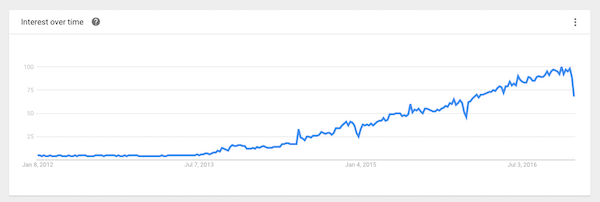
\includegraphics[height=4.2cm]{imagens/docker}
\caption{Gráfico de utilzação do docker entre os anos 2012 e 2016.}
\label{fig:utilizacao-docker}
\end{figure}

A velocidade do micro-serviço permite e incentiva a implementação e estudo dos mesmos. Segundo Adrian (Membro e fundador da eBay Research Labs)  micro-serviços possui características comum, como: Implantação com pouca frequência, novas versões implantadas automaticamente, orquestração de uso geral não é necessário, uma vez que, sistemas inteiros são implantados com todas as partes ao mesmo tempo, arquiteturas utilizam centenas de micro-serviços e cada publicação é altamente customizada.
Seguindo adiante, o próximo passo que Adrian vê é orquestração para aplicações baseadas em padrões portáteis, em vez de dezenas de micro-serviços nas quais novas versões são automaticamente implantadas e que escalabilidade e disponibilidade são asseguradas, prevendo também um movimento contínuo de arquiteturas monolíticas para arquiteturas de micro-serviços. (STENBERG, 2015).

Implantar a Arquitetura de micro-serviços em empresas vai proporcionar diferentes benefícios para a estrutura de negócio como: usufruir de liberdade maior para o desenvolvimento de serviços de modo independente, implantar automaticamente através de ferramentas de integração contínua e código aberto, como Hudson, Jenkins e outras, possibilitar utilização de códigos escritos em linguagens diferentes para diferentes serviços utilizando comunicação REST através de Json ou XML, facilitar a ampliação e integração de micro-serviços com serviços terceirizados, através de APIs, organizar o código em função de capacidades de negócio, dando mais visão das ofertas e necessidades dos clientes. Dentre todos os benefícios citados é possível fazer o gerenciamento otimizado de falhas, o que significa que, se um serviço venha a falhar, os outros continuarão funcionando. Através dos micro-serviços, é possível identificar falhas com mais eficiência, visto que o particionamento favorece uma visão mais detalhada de cada serviço (PELOI, 2016). É possível observar na figura \ref{fig:art-scalability} as três dimensões da escalabilidade, onde o eixo X refere-se à escalabilidade horizontal, para ampliar a capacidade e disponibilidade da aplicação (cada servidor executa uma cópia idêntica do código), Z semelhante à do eixo X,  mas requer a presença de um componente que se responsabilize pelo roteamento das requisições ao servidor adequado, e o eixo Y que representa a terceira dimensão da escalabilidade, denominada decomposição funcional e é responsável por dividir a aplicação em uma série de serviços. A cada serviço corresponde um conjunto de funções (gerenciamento de pedidos, gerenciamento de clientes, entre outros).

\begin{figure}[h]
\centering
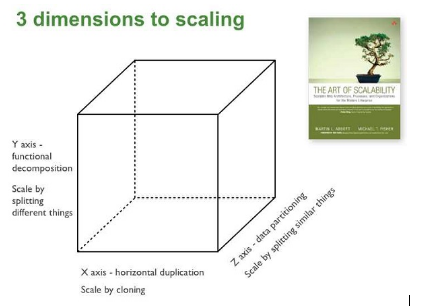
\includegraphics[height=6.2cm]{imagens/scalability}
\caption{The Art of Scalability - 2009.}
\label{fig:art-scalability}
\end{figure}


Segundo dados de Richardson(2014), diversas empresas estão utilizando micro-serviços, dentre as citadas estão: Comcast Cable, Uber, Netflix, Amazon, Ebay, SoundCloud, Karma, Groupon, Hailo, Gilt, Zalando, Lending Club, AutoScout24.
Os problemas associados ao desenvolvimento de software em larga escala ocorreram em torno da década de 1960. Na década de 1970 viu-se um enorme aumento de interesse da comunidade de pesquisa para o design de software em suas aplicações e  no processo de desenvolvimento. Nesta década o design foi muitas vezes considerado como uma atividade não associada com a implementação em si, e portanto requerendo um conjunto especial de notações e ferramentas. Por volta da década de 1980, a integração do design nos processos de desenvolvimento contribuiu para uma fusão parcial dessas duas atividades, tornando assim mais difícil fazer distinções puras.

As referências ao conceito de arquitetura de software também começaram a aparecer década de 1980. No entanto, uma base sólida sobre o tema foi estabelecida apenas em 1992 por Perry Wolf (autor do livro “Foundations for the study of software architecture"). Sua definição de arquitetura de software era distinta do design de software, e desde então tem-se gerado uma grande comunidade de pesquisadores estudando as aplicações práticas da arquitetura de software com base em micro-serviços, permitindo  assim que os conceitos sejam amplamente adotados pela indústria e pela academia.

O advento e a difusão da orientação por objetos, a partir dos anos 80 e, em particular, a década de 1990, trouxe sua própria contribuição para o campo da Arquitetura de Software. O clássico por Gamma et ai. abrange a concepção de software orientado a objetos e como traduzi-lo em código que apresenta uma coleção de soluções recorrentes, chamados padrões. Esta ideia não é nova nem exclusiva à Engenharia de Software, mas o livro é o primeiro compêndio a popularizar a idéia em grande escala. Na era pré-Gamma os padrões para soluções OO já estavam sendo utilizado: um exemplo típico de um padrão de projeto arquitetônico em programação orientada a objetos é o Model-View-Controller (MVC), que tem sido um dos insights seminais no desenvolvimento precoce de interfaces gráficas de usuário.(DRAGONI et al., 2016)

Cerca de sete anos atrás a empresa Netflix (provedora global de filmes e séries de televisão via streaming - distribuição de dados, geralmente de multimídia em uma rede através de pacotes) começou a migrar suas aplicações legadas para uma arquitetura baseada em APIs (Interface de programação de aplicativos) hospedadas na nuvem (local para armazenamento de dados online) da Amazon (empresa transnacional de comércio electrónico dos Estados Unidos com sede em Seattle), influenciando assim, o crescimento de uma ideologia na área de desenvolvimento de softwares que foi batizada pelo nome de “micro-serviço”.

Uma investigação realizada pela empresa Cisco (Companhia sediada em San José, Califórnia, Estados Unidos da América) em 2016 revela que, apesar de toda a euforia sobre a Internet das Coisas, o consumo de de vídeo via internet gera 63\% do tráfego global. A expectativa é que essa marca chegue a 79\% até 2020 e o tráfego de dados gerado por vídeos em resolução Ultra HD subirá de 1.6\% para 20.7\% do total em 2020. Um levantamento realizado pela Cisco VNI Mobile 2016 mostra que os dispositivos IoT mais simples geram uma quantidade de dados equivalentes a 7 veze o que é produzido por um celular comum (não um smartphone). Demandando pouco das redes de telecomunicações, os dispositivos IoT não representarão um grande pessoa para os provedores de infraestrutura na América Latina (IDC, 2016). 

Segundo o relatório “The State of Internet” de 2016, da Akamai (Empresa de Internet americana, sediada em Cambridge, Massachusetts), o país melhor colocado na faixa de redes com banda igual ou maior a 15 Mb/s é o Chile - 4,4\% de seus serviços de Internet atingem essa marca. Entretanto, para chegar a essa posição, o Chile investiu pesadamente entre 2014 e 2015, conseguindo crescer 150\% de um ano para outro. O Uruguai fica logo abaixo, com 4,1\% de sua Internet na faixa dos 15 Mb/s. Atualmente no Brasil, somente 1,1\% dos serviços atingem esta marca.

Na arquitetura de microserviços, se quisermos que um aplicativo seja colocado em esteróides, ele pode ser feito sem afetar outros serviços. Podemos apenas começar a executar este serviço específico em um hardware mais forte. Um microservice único pode ser atualizado nesta arquitetura, sem afetar outros ... a única condição é que o sistema de tempo de execução suporta isso. Cada microservice em uma plataforma pode ser desenvolvido em uma linguagem diferente - Java, C, C ++, Python, etc Governança granular é possível para cada microservice porque não tem dependência em outro. Ele pode ser monitorado e governado separadamente. Essa arquitetura descentraliza o gerenciamento de dados, uma vez que cada microserviço pode armazenar seus dados de uma maneira que se adapte a ele. Arquitetura Microservice suporta automação. É possível mover montagens inteiras de microservices de um ambiente de implementação para outro apenas usando as configurações de perfil com um único clique. Eles são muito mais resistentes do que as aplicações tradicionais. Isto é devido ao fato de que uma única aplicação pode ser retirada de um monte de aplicativos microservices, como estes são independentes uns dos outros.

A arquitetura do microservice tem suas vantagens óbvias e aquela é a razão porque assim que muitos negócios e serviços públicos proeminentes como Netflix, eBay, Amazon, o serviço digital do governo BRIT NICO, realestate.com.au, para diante, Twitter, Paypal, Gilt, Bluemix, Soundcloud , The Guardian, etc, apenas para citar alguns, todos se graduaram de arquitetura monolítica a microservices. Embora este seja o caso, assim como não há um plano perfeito, não há nenhuma arquitetura perfeita. O que funciona sob uma circunstância particular pode se tornar o gargalo em outro.

\subsection{Tecnologias}
Neste trabalho será utilizado no Back-end a tecnologia do netflix Service Discovery (Eureka), e para comunicar com este serviço será utilizado o circuito integrado Nodemcu Esp8266. Existem outras bibliotecas que podem trabalhar em conjunto com o Eureka que são: Circuit Breaker (Hystrix), Intelligent Routing (Zuul) and Client Side Load Balancing (Ribbon). 

\subsubsection{Zuul}
Zuul é a “porta da frente” para todas as requisições de dispositivos e sites para o back-end. O mesmo foi construído para permitir roteamento dinâmico, monitoramento, resiliência e segurança. O Zuul foi desenvolvido pela Netflix pelo fato de que o volume e a diversidade do tráfego da API do mesmo resultam em problemas de produção que surgem rapidamente e  sem aviso prévio, eles precisavam de um sistema que permita os mesmos mudar rapidamente o comportamento e reagir a estas situações.
O Zull utiliza uma variedade de diferentes tipos de filtros que permite-se aplicar rapidamente funcionalidades os serviços de ponta. Esses filtros ajudam a executar as seguintes funções: Autenticação e segurança, identificando requisitos de autenticação para cada recurso e rejeitando solicitações indesejadas. Insights e monitoramento, rastreamento de dados significativos e estatísticas, a fim de dar uma visão precisa da produção. Roteamento dinâmico, encaminhado dinamicamente solicitações para diferentes clusters de backend conforme necessário. Stress Testing, aumento gradual de tráfego para um cluster, a fim de avaliar o desempenho. Load Shedding, alocação de capacidade para cada tipo de solicitação e soltando pedidos que excedem o limite. Manipulação de resposta estática, construção de respostas diretamente na ponta ao invés de encaminhá-las para um cluster interno.
Dentre os vários componentes que integram a biblioteca do Zuul, estão: Zuul-core que contém funcionalidades a fim de compilar e executar filtros, Zuul-simple que mostra como construir um aplicativo com zuul-core, Zuul-netflix que adiciona componentes Netflix utilizando Ribbon para solicitações de roteamento. (Zuul, 2014)

\subsubsection{Ribbon}
Ribbon dá suporte à comunicação entre processos na nuvem e inclui balanceadores de carga desenvolvidos pela netflix. A tecnologia citada fornece os seguintes recursos: regras de balanceamento de carga múltiplas e conectáveis, integração com a descoberta de serviços, resiliência de falhas incorporada, clientes integrados com balanceadores de carga e configuração de clientes utilizando Archaius. O Ribbon é composto pelos seguintes projetos: Ribbon-core que inclui definições de interface e balanceamento de carga e cliente, implementações de balanceador de carga comuns, integração de cliente com balanceadores de carga e fábrica de clientes. Ribbon-eureka que inclui implementações do balanceador de carga com base no Eureka-client (bibliote para registro e descoberta de serviços). Ribbon-httpclient que inclui a inclui a implementação baseada em JSR-311 do cliente REST integrada com balanceadores de carga.

\subsubsection{Hystrix}
Hystrix é um ambiente distribuído, inevitavelmente algumas das muitas dependências de serviços falharão, e esta biblioteca ajuda a controlar as interações entre serviços distribuídos adicionando tolerância de latência e lógica de tolerância a falhas. O mesmo faz isso isolando pontos de acesso entre os serviços, interrompendo falhas em cascata através deles, todas as quais melhoram a resiliência geral do sistema. Atualmente, dezenas de bilhões de threads isoladas e centenas de bilhões não isoladas são executadas utilizando o Hystrix todos os dias na Netflix. Isso resulta em uma melhoria dramática no tempo e atividade e resiliência. Hystrix é projeto para: proteger e controlar a latência e falhas de dependências acessadas por meio de bibliotecas de terceiros, interromper falhas em cascata em um sistema distribuído, recuperação rápida a falhas, monitoramento em tempo real, alertas e controle operacional. Quando se trata de micro-serviços, os mesmos contém dezenas de dependências com outros micro-serviços, o que ocasiona que se um deles falhar e o mesmo não estiver isolado destas falhas externas, corre o risco de também ser afetado. Por exemplo, um aplicativo que dependa de 40 serviços em que cada serviço tem 99,99\% de disponibilidade, pode se esperar: 99,99 \^ 40 = 99,6\% de tempo de atividade, 0.4\% de 1 bilhão de falhas resulta em 4 milhões de falhas. Mesmo que pequena a possibilidade de falha, se somar a quantidade de micro-serviços ao tempo de indisponibilidade que pode surgir por pequenas falhas, o problema pode ser facilmente escalável fazendo com que assim serviços importantes fiquem até mesmos horas indisponíveis. Quando toda a aplicação está funcionando e configurada de maneira correta, o fluxo de solicitações ocorrer conforme a figura \ref{fig:hystrix-overtime}.

\begin{figure}[h]
\centering
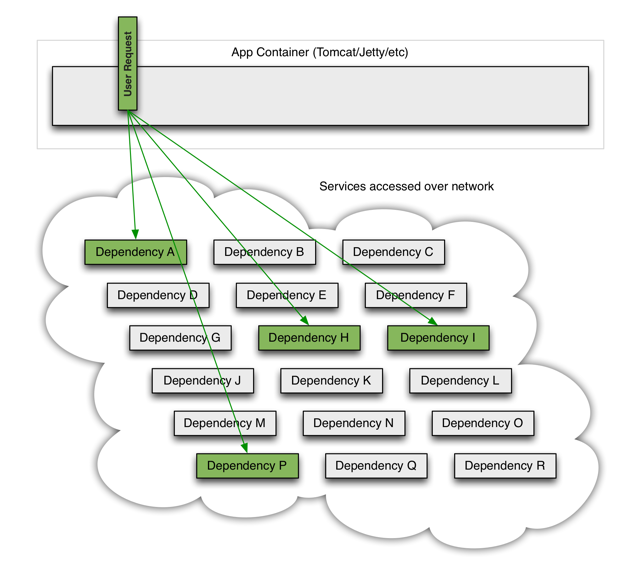
\includegraphics[height=6.2cm]{imagens/figura3}
\caption{Wiki Hystrix (Internet Overtime) - 2015).}
\label{fig:hystrix-overtime}
\end{figure}

Quando um dos muitos serviços se torna latente, ele pode bloquear toda a solicitação do usuário, conforme apresentado na figura \ref{fig:hystrix-dimensions-scaling}.

\begin{figure}[h]
\centering
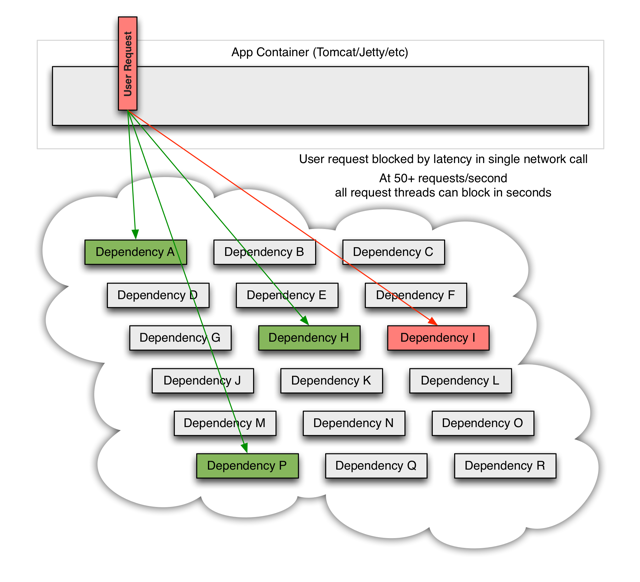
\includegraphics[height=6.2cm]{imagens/figura4}
\caption{Wiki Hystrix (3 dimensions to scaling) - 2015).}
\label{fig:hystrix-dimensions-scaling}
\end{figure}

Com tráfego de alto volume, uma única dependência com latência excessiva, pode fazer com todos os recursos fiquem saturados em segundo. Cada ponto em um aplicativo que atinge a rede ou em uma biblioteca cliente que pode resultar em solicitações de rede é uma fonte de falha potencial. Pior que falhas, esses aplicativos também podem resultar em latências aumentadas entre os serviços, que faz backup de filas e outros recursos do sistema, causando ainda mais falhas em cascata em todo a aplicação, conforme a figura \ref{fig:hystrix-container}.

\begin{figure}[h]
\centering
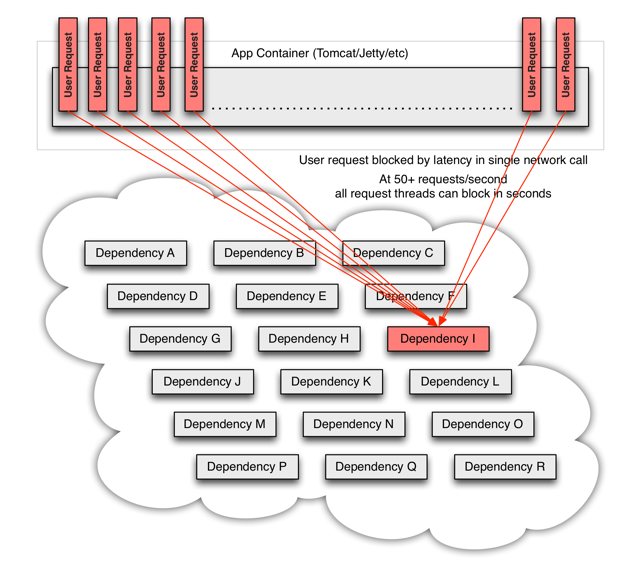
\includegraphics[height=6.2cm]{imagens/figura5}
\caption{Wiki Hystrix (Container) - 2015).}
\label{fig:hystrix-container}
\end{figure}

A biblioteca Hystrix subjaz os seguintes princípios de design: Impedir que qualquer dependência única utilize todos as threads de usuários de container (como Tomcat), desperdiçando carga, fornecer soluções sempre que possível para proteger os usuários contra falhas, utilizando técnicas de isolamento para limitar o impacto de qualquer dependência, otimizar o tempo de descoberta através de métricas, monitoramento e alertas em tempo quase real, otimizando o tempo de recuperação por meio de propagação de baixa latência de alterações de configuração e suporte para alterações de propriedade dinâmicas na maioria dos aspectos do Hystrix, o que permite fazer modificações operacionais em tempo real com loops de realimentação de baixa latência, protegendo contra falhas em toda a execução do cliente de dependência, não apenas no tráfego da rede. (Hystrix, 2015)

\subsubsection{Eureka + Spring Cloud}
Spring Cloud fornece integrações Netflix OSS para Spring Boot por meio de auto-configuração e vinculação ao Spring Environment e outros padrões de programação Spring. Dentre os produtos spring Cloud encontra-se os clientes Eureka ou Service Discovery que é um dos princípios fundamentais de uma arquitetura baseada em micro-serviços. Configurar um micro-serviço é trabalhado pois envolve diversas técnicas de descoberta e registro de serviços, e com o Service Discovery da Netflix torna-se eficiente este trabalho pois com poucas anotações Java consegue-se criar uma aplicação simples Eureka. 

Eureka também vem com um componente de cliente baseado em Java, o cliente Eureka, que torna as interações com o serviço muito mais fácil. Ocliente também tem um balanceador de carga incorporado que faz balanceamento de carga round-robin (Algoritmos simples de agendamento e escalonamento de processos) básico. Quando um cliente se registra no mesmo, o mesmo fornece metadados sobre, como host e porta, dentre outras informações que podem ser encontradas na documentação. Se o registro falhar durante a configuração, a instância da aplicação é removida do registro. Em resumo, o Eureka é um serviço baseado em REST (Representational State Transfer) que é utilizado principalmente na AWS (Amazon Web Services) para localizar serviços com a finalidade de balanceamento de carga e failover (tolerância a falhas) de servidores de camada intermediária. 

A Amazon possui um produto chamado AWS ELB (Amazon Web Services Elastic Load Balancer), que é uma solução de balanceamento de carga para serviços de ponta expostos ao tráfego web do usuário final, e a diferença entre o mesmo e o produto da Netflix, é que o Eureka preenche a necessidade de balanceamento de carga médio. Embora teoricamente pode-se colocar serviços de nível intermediário atrás do AWS ELB, no EC2 classic (Elastic Compute Cloud) pode-se expor ao mundo exterior e perder toda a utilidade dos grupos de segurança AWS. O AWS ELB  também possui uma solução de balanceamento de carga em proxy (servidor intermediário para requisições entre cliente e servidor final) tradicional, enquanto no Eureka, o balanceamento ocorre no nível da instância, servidor e host. As instâncias do cliente sabem todas as informações sobre quais aplicações precisam conversar.

Uma questão a ser analisada no Eureka, é o DNS (Domain Name System). Dentre as aplicações existente para resolução de DNS está o Route 53, um serviço de nomeação, como o qual Eureka pode fornecer o mesmo para os servidores de nível médio. Route 53 é um serviço DNS e também pode fazer roteamento baseado em latência em regiões AWS. Eureka é análogo ao DNS interno e não tem nada a ver com os servidores DNS em todo o mundo. Eureka também é isolado no sentido de que não sabe sobre servidores em outras regiões AWS. Sua finalidade principal de manter informações é para balanceamento de carga dentro de uma região.

Na Netflix, além de desempenhar um papel crítico no balanceamento de carga de nível médio, o Eureka é utilizado para os seguintes fins: implementações com Netflix Asgard, um serviço para fazer atualizações de serviços de forma rápida e segura, registro e exclusão de instâncias e transporte de metadados específicos de aplicativos adicionais sobre serviços. Dentre os motivos para utilizar o Eureka está o fato que o mesmo provê uma solução para balanceamento de carga round-robin simples, e quem não estiver disposto a se registrar com o AWS ELB e expor seu tráfego externamente, o mesmo resolve este problema.

Com o Eureka, a comunicação é transparente, pois o mesmo fornece informações sobre os serviços desejados para comunicação, mas não impõe quaisquer restrições sobre o protocolo ou método de comunicação. Exemplificando, pode-se utilizar o Eureka para obter o endereço do servidor destino e utilizar protocolos como thrift, http (s) ou qualquer outro mecanismos RPC (Remote Procedure Call) que permite fazer conexões ou chamadas por espaço de endereçamento de rede. 

\subsubsection{Modelo Arquitetural Eureka}
O modelo arquitetural implantado na Netflix utilizando o Eureka é  descrita na figura \ref{fig:wiki-eureka-est}. Existe um cluster por região que conhece somente instâncias de sua região. Há pelo menos um servidor Eureka por zona para lidar com falhas da mesma. Os serviços se registram e, em seguida, a cada 30 segundos enviam os chamados “batimentos cardíacos” ou requisições para renovar seus registros. Se o cliente não renovar o registro, ele é retirado do servidor em cerca de 90 segundos. As informações de registro e renovações são replicadas para todos as conexões no cluster. Os clientes de qualquer zona podem procurar as informações do registro para localizar seus serviços que podem estar em qualquer zona e fazer chamadas remotas.

Para serviços não baseados em Java, tem-se a opção de implementar a parte do cliente utilizando o protocolo REST desenvolvido para o Eureka ou executar um “side car” que é uma aplicação Java com um cliente embutido Eureka que manipula os registros e conexões. Quando se trabalha com serviços em nuvem, pensar em resiliência se torna ímprobo. Eureka se beneficia dessa experiência adquirida, e é construído para lidar com falha de um ou mais servidores do mesmo.

\begin{figure}[h]
\centering
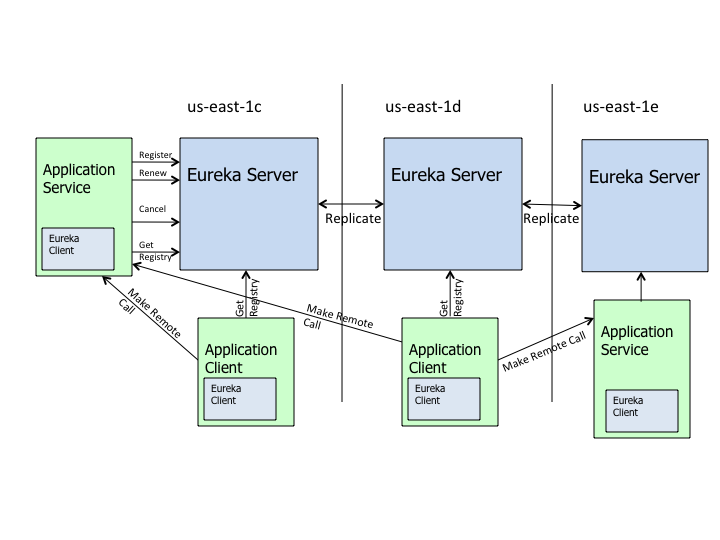
\includegraphics[height=6.2cm]{imagens/figura6}
\caption{Wiki Eureka - 2015).}
\label{fig:wiki-eureka-est}
\end{figure}







% Exemplo tabela
% \begin{table}[h]
% \centering
% \caption{ Modelo de como as tabelas devem ser inseridas no texto }
% \vspace{0.2in}
% \newcolumntype{C}{>{\centering\arraybackslash}X}%
% \newcommand{\rowstyle}[1]{%
%   \protected\gdef\currentrowstyle{#1}%
% }
% \begin{tabularx}{\textwidth}{>{\bf}C|C|C|C}
% \hline 
% \textbf {Índice} & \textbf{Coluna 01} &\textbf{ Coluna 02} & \textbf{Coluna 03} \\ \hline \hline
% Linha 01 & & & \\ \hline
% Linha 02 & & & \\ \hline                         

% \end{tabularx}
% \end{table}

% \section{DESENVOLVIMENTO}

\subsection{Introdução ao Eureka}

Neste trabalho tem-se por objetivo o a pesquisa e desenvolvimento de uma estrutura IoT baseado no padrão de micro-serviços, e para isto precisa-se utilizar um dos princípios que foi citada na revisão bibliográfica que é o "Service Discovery" ou descoberta de serviços. Como o projeto será baseado em Java, inicialmente será criado um projeto e  utilizará maven para gerenciamento de dependências e o Eureka Client para descoberta de serviços. Para poder utilizar o maven deve-se criar um arquivo de configurações no diretório raíz do projeto chamado "pom.xml", e a documentação completa pode se encontrar no site de seus desenvolvedor. Posteriormente será incluso o seguinte groupId org.springframework.cloud e o artifactId spring-cloud-starter-eureka, e para mais informações pode ser encontrada na documentação oficial do Spring Cloud Netflix.

Quando um cliente se registra com o Eureka, ele fornece meta-dados sobre si, indicador de estado ou saúde, página inicial, dentre outros. Eureka recebe mensagens heartbeat (disponibilidade) de cada instância pertencente a um serviço. Se algum heartbeat falhar, a instância é removido do registro.
Para inicializar um projeto com Eureka Client, será utilizado algumas anotações Java fornecidas pelo Eureka descritas a seguir: @Configuration, para utilizar recursos do projeto Spring Config para facilitar configurações de projetos Spring baseado em Java, @ComponentScan para buscar componentes em pacotes java, @EnableAutoConfiguration para ativar a ComponentScandescritas a seguir: @EnableEurekaClient para ativar a descoberta de serviços do Eureka, @RestController para criar um controlador Rest (Representational State Transfer), @RequestMapping para mapear as rotas da aplicação.

\begin{verbatim}
@Configuration
@ComponentScan
@EnableAutoConfiguration
@EnableEurekaClient
@RestController
public class Application {

    @RequestMapping("/")
    public String home() {
        return "Hello world";
    }

    public static void main(String[] args) {
        new SpringApplicationBuilder(Application.class)
          .web(true).run(args);
    }
}
\end{verbatim}

Para que possa surtir efeito na aplicação precisa fazer ajustes nas configurações do Eureka dentro do diretório resources da aplicação Java. Esta configuração é feita dentro de um arquivo Application.yml.

\begin{verbatim}
  Eureka
   cliente:
     ServiceUrl:
       DefaultZone: http: // localhost: 8761 / eureka / 
\end{verbatim}

Neste arquivo de configuração encontra-se uma peculariedade. O DefaultZone é a URL do serviço Eureka para qualquer cliente. O nome do aplicativo padrão (ID de serviço), o host e a porta podem ser acessadas respectivamente pelas variáveis de ambientes: \${spring.application.name} , \${spring.application.name} e \${server.port}.
A anotação Java @EnableEurekaClient faz com que o a aplicação corrente se registre no Eureka, para que assim possa localizar outros serviços.

\subsection{Status e Saúde do serviço}

Com a página de status e os indicadores de integridade de uma instância do Eureka é possível visualizar informações do serviço. Para acessar os indicadores de saúde deve-se configurar as rotas padrões de acesso a mesma. Por padrão, o eureka utiliza a conexão do cliente para determinar se um cliente está ativo. Caso não utilize o Discovery Client, não será propagado o status de verificação de integridade atual do serviço. Para funcionar corretamente os indicadores de saúde e status da aplicação, devem ser feitas as seguintes configurações:

\begin{verbatim}
eureka:
  instance:
    statusPageUrlPath: ${management.context-path}/info
    healthCheckUrlPath: ${management.context-path}/health
  client:
    healthcheck:
      enabled: true
\end{verbatim}

Para conseguir utilizar mais recursos e obter mais informações sobre o status da aplicação, a aplicação deve implementar seu próprio controle de integridade que se encontra no pacote com.netflix.appinfo.HealthCheckHandler

\subsection{Alterando o ID da instância Eureka}

Uma instancia registrada no Eureka possui seu ID, que identifica o serviço que está no mesmo. O Spring Cloud Eureka fornece o seguinte padrão de configuração: \$\{spring.cloud.client.hostname\}:\$\{spring.application.name\}:\$\{spring.application.instance\_id:
\$\{server.port\}\}. Como exemplo a URL fica da seguinte maneira: myhost:myapp:8080

\subsection{EurekaClient}

O próximo passo para aprender a utilizar os clientes Eureka, é aprende a utlizar o EurekaClient, que pode ser utilizado para descobrir instâncias do Eureka Server. Para fazer isto utilizando o framework desenvolvido para Java pela Spring Cloud, precisa primeiramente injetar a dependência do EurekaClient e criar um método que busque as instâncias registradas no Eureka.

\begin{verbatim}
@Autowired
private EurekaClient discoveryClient;

public String serviceUrl() {
    InstanceInfo instance = 
      discoveryClient.getNextServerFromEureka("STORES", false);
    return instance.getHomePageUrl();
}
\end{verbatim}

Não necessariamente precisa utilizar o EurekaClient. Também pode-se utilizar o DiscoveryClient. A diferença entre os dois, está na maneira de como é utilizado.

\begin{verbatim}
@Autowired
private DiscoveryClient discoveryClient;

public String serviceUrl() {
    List<ServiceInstance> list = 
      discoveryClient.getInstances("STORES");
    if (list != null && list.size() > 0 ) {
        return list.get(0).getUri();
    }
    return null;
}
\end{verbatim}

\subsection{Performanece de registro no Eureka}

Registrar um serviço no Eureka pode ser considerado um pouco lento, pelo fato de que ser uma instância também envolve um heartbeat periódico para o registro com duração padrão de 30 segundos. Um serviço não estará disponível para descoberta por clientes enquanto uma intância tenha todos os metadados em seu cache local. Para alterar o período em que isto ocorre pode ser configurado através da propriedade eureka.instance.leaseRenewalIntervalInSeconds. Entretanto, em produção, não deve ser alterado este padrão pelo fato de que, existem alguns cálculos internos do Eurela que fazem suposições de renovação de locação.

\subsection{Zonas Eureka}

Primeiramente, para se configurar uma zona Eureka, precisa-se ter certeza de que existem servidores Eureka implantados em cada zona e que eles são pares uns dos outros. Em seguida, precisa-se informar em qual zona o mesmo está. Para fazer isto será utilizado a propriedade metadataMap. E isto pode ser feito da seguinte forma:

\begin{verbatim}
eureka.instance.metadataMap.zone = zone1
eureka.client.preferSameZoneEureka = true
\end{verbatim}

\subsection{Primeiros passos com Eureka Server}

Primeiramente, para começar a utilizar o Eureka, como este projeto é baseado em Java no backend e utiliza maven como gerenciador de dependências, deve ser incluido nas mesmas a dependência com o groupId org.springframework.cloud e o artifactId spring-cloud-starter-eureka-server. Com esta dependência adicionada, será possível utilzar o Eureka Server.

Após adicionar esta dependência, deve ser criado a classe principal que se encarregará de iniciar a aplicação Eureka Server. Utilizando-se da anotação @EnableEurekaServer fornecida pelo framework e seguindo o padrão utilizado no Eureka Client para iniciar a aplicação, é possível ver um resultado. Um exemplo de código pode ser visto a seguir.

\begin{verbatim}
@SpringBootApplication
@EnableEurekaServer
public class Application {

    public static void main(String[] args) {
        new SpringApplicationBuilder(Application.class).web(true).run(args);
    }

}
\end{verbatim}

\subsection{Modo Autônomo}

A combinação entre o cliente e servidor Eureka e as pulsações para verificação de disponibilidade entre os mesmos, tornam o servidor Eureka Autônomo bastante resiliente à falha, contanto que haja algum tipo de monitoramento para mantê-lo funcionando. No modo autônomo, pode-se prefirir desativar o comportamento padrão do lado do cliente, para que ele não continue tentado alcançar seus pares caso haja falha. Para isto será feito diversas configurações como pode ser visto a seguir.


\begin{verbatim}
server:
  port: 8761

eureka:
  instance:
    hostname: localhost
  client:
    registerWithEureka: false
    fetchRegistry: false
    serviceUrl:
      defaultZone: http://${eureka.instance.hostname}:${server.port}/eureka/
\end{verbatim}

Acima foi apresentado as seguintes configurações: port que configura a porta em que será instalado a aplicação, hostname para identificar o nome do host, registerWithEureka que indica se a própria aplicação do Eureka se registra em si mesma e fetchRegistry que diz se o Eureka buscará registros associados a eles que ainda estão executando, porém ainda não registradas no Eureka.
Com o Eureka, os registros podem ser ainda mais resistentes e disponíveis executando várias instâncias e pedindo-lhes para se registrarem uns com os outros. Tudo o que precisa para fazê-lo é configurar o serviceUrl dos pares.

\begin{verbatim}
---
spring:
  profiles: peer1
eureka:
  instance:
    hostname: peer1
  client:
    serviceUrl:
      defaultZone: http://peer2/eureka/

---
spring:
  profiles: peer2
eureka:
  instance:
    hostname: peer2
  client:
    serviceUrl:
      defaultZone: http://peer1/eureka/
\end{verbatim}

Neste exeplo, temos configurado, que o serviço pode ser utilizado para executar o mesmo servidor em 2 hosts (peer1 e peer2), executando-o em diferentes perfis Spring. Pode-se utilizar esta configuração para testar a descoberta dos pares em um único host, manipulando se em servidor Linux o arquivo hosts para resolver os nomes de host que pode ser encontrado dentro do diretório /etc/hosts.

Em alguns casos, é preferível que o Eureka utilize os endeços IP dos serviços ao invés do nome do host. Para isto deve ser definido a configuração eureka.instance.preferIpAddress como true e quando a aplicação se registrar com o Eureka, o mesmo utilizará seu endereço IP ao invés de seu nome de host.

\subsection{Clientes Hystrix}

Segundo Fowler (2016) é comum que os sistemas de software façam chamadas remotas para software em execução em diferentes processos, provavelmente em máquinas diferentes em uma rede. Uma das grandes diferenças entre chamadas em memória e chamadas remotas é que chamadas remotas podem falhar ou travar sem uma resposta até que algum limite de tempo limite seja atingido. O que é pior se você tem muitos chamadores em um fornecedor que não responde, então você pode ficar sem recursos críticos levando a falhas em cascata em vários sistemas. Em seu excelente livro Release It  , Michael Nygard popularizou o padrão de disjuntor para evitar este tipo de cascata catastrófica.

Com todos estes problemas que podem ocorrer na arquitetura de micro-serviços, a Netflix criou a biblioteca chamada Hystrix, que impelementa o padrão disjuntor que interromple automáticamente o serviço quando ocorre falhas. Uma falha de serviço no nível inferior de serviços pode causar falha em cascata em todo o caminho até o usuário. No Hystrix o padrão de limite de falhas são 20 em 5 segundos, e quando ocorre o circuito é aberto e a chamada não é feita, isto pode ser visto na figura \ref{fig:figura7}

\begin{figure}[h]
\centering
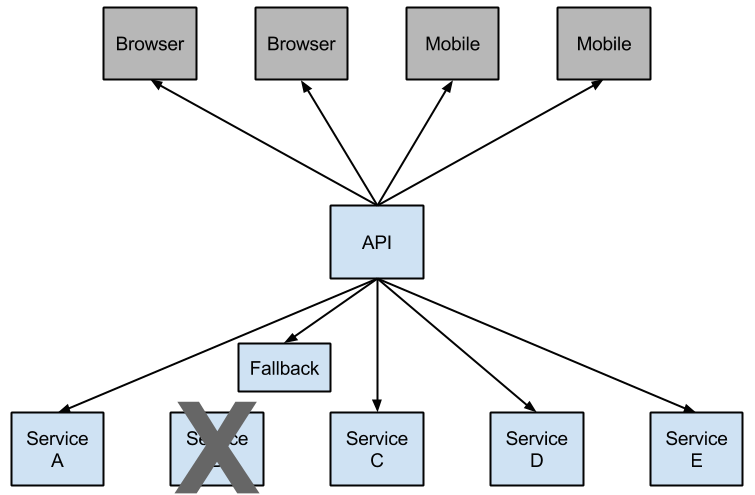
\includegraphics[height=4.2cm]{imagens/figura7}
\caption{Fallback Hystrix em falhas em cascata.}
\label{fig:figura7}
\end{figure}

\subsection{Primeiros passos com Hystrix}

Para utilizar o Hystrix, precisa seguir o mesmo padrão de quando se começa uma aplicação Eureka Server ou Client. No caso do padrão deste projeto backend baseado em Java com gerenciado de dependências maven, o que mudará será a anotação utilizada na classe principal do projeto e a dependência maven utilizada. Para incluir no projeto, será utilizado a dependência com o groupId org.springframework.cloud e o artifactId spring-cloud-starter-Hystrix, e a anotação @EnableCircuitBreaker na classe principal.

\begin{verbatim}
@SpringBootApplication
@EnableCircuitBreaker
public class Application {

    public static void main(String[] args) {
        new SpringApplicationBuilder(Application.class).web(true).run(args);
    }

}

@Component
public class StoreIntegration {

    @HystrixCommand(fallbackMethod = "defaultStores")
    public Object getStores(Map<String, Object> parameters) {
        //do stuff that might fail
    }

    public Object defaultStores(Map<String, Object> parameters) {
        return /* something useful */;
    }
}
\end{verbatim}

No exemplo de código acima, foi implementando uma classe que se contém um método que buscara os serviços, e para isto foi utilizado a anotação @HystrixCommand.

É possível ativar as métricas Hystrix e a central de gerenciamento do mesmo adicionando as dependências abaixo. O endpoint para acesso ao gerenciador é /hystrix.stream.

\begin{verbatim}
<dependency>
    <groupId>org.springframework.boot</groupId>
    <artifactId>spring-boot-starter-actuator</artifactId>
</dependency>
<dependency>
    <groupId>org.springframework.cloud</groupId>
    <artifactId>spring-cloud-starter-hystrix-dashboard</artifactId>
</dependency>
\end{verbatim}

\subsection{Ribbon}

Ribbon é um  balanceador de carga do lado do cliente que fornece controles sobre o comportamento dos clientes HTTP e TCP. Uma observação importante é que a anotação @FeignClient já utiliza Ribbon, fazendo com que assim seja desnecessário a utilização do Ribbon, entretanto, quando for preciso um controle mais versátil sobre a tecnologia é optável a utilização do mesmo.

Para incluir o ribbon no projeto, será utilizado o mesmo padrão de configurações feito anteriormente. O que será alterado é a o artifactId da dependência maven que agora será utilizado spring-cloud-starter-ribbon, e para configurar o cliente Ribbon criado uma classe de configuraçao e será anotado com @RibbonClient. 

\begin{verbatim}
@Configuration
@RibbonClient(name = "foo", configuration = FooConfiguration.class)
public class TestConfiguration {
}
\end{verbatim}

\subsection{FeignClient}

FeignClient é uma biblioteca que faz com que clientes de serviços web sejam escritos de forma mais fácil. Para utilizá-lo é preciso instalar a dependência spring-cloud-starter-feign e anotar a classe principal com @EnableFeignClients. O mesmo provê suporte para anotações Spring MVC e por utilizar o mesmo conversor de mensagens HTTP que o Spring Web, é integra com Hystrix para fornecer um cliente com balanceamento de carga.

\begin{verbatim}
@Configuration
@ComponentScan
@EnableAutoConfiguration
@EnableEurekaClient
@EnableFeignClients
public class Application {

    public static void main(String[] args) {
        SpringApplication.run(Application.class, args);
    }

}
\end{verbatim}

Ao anotar uma interface com @FeignClient, pode ser mapeado os métodos para que consiga acesso a endpoints da biblioteca. O nome do método será qualificado e aplicado ao contexto da aplicação, fazendo com que assim não seja implementado corpo ao método pois será apenas repassados chamadas REST.

\begin{verbatim}
@FeignClient("stores")
public interface StoreClient {
    @RequestMapping(method = RequestMethod.GET, value = "/stores")
    List<Store> getStores();

    @RequestMapping(method = RequestMethod.POST, value = "/stores/{storeId}", consumes = "application/json")
    Store update(@PathVariable("storeId") Long storeId, Store store);
}
\end{verbatim}

Cada Cliente Feign faz parte de um conjunto de componentes que trabalham juntos para comunicar-se via HTTP. O Spring Cloud permite com que se tenha controle total sobre clientes Feign declarando uma classe de configuração que implemente determinados métodos do FeignClient. Duas das possíveis configuração, sao: modificar o padrão de Contrato que o FeignClient utiliza para que assim seja personalizado o padrão de comunicação REST que o mesmo utiliza e modificar o método de autenticação do FeignClient.

\begin{verbatim}
@Configuration
public class FooConfiguration {
    @Bean
    public Contract feignContract() {
        return new feign.Contract.Default();
    }

    @Bean
    public BasicAuthRequestInterceptor basicAuthRequestInterceptor() {
        return new BasicAuthRequestInterceptor("user", "password");
    }
}
\end{verbatim}

Em alguns casos, pode ser necessário outros métodos mais especificos para que seja personalizado as configurações. Neste caso, pode-se utilizar a API Feign Builder. Abaixo está um exemplo da utilização do mesmo.

\begin{verbatim}
@Import(FeignClientsConfiguration.class)
class FooController {

	private FooClient fooClient;

	private FooClient adminClient;

    @Autowired
	public FooController(
			Decoder decoder, Encoder encoder, Client client) {
		this.fooClient = Feign.builder().client(client)
				.encoder(encoder)
				.decoder(decoder)
				.requestInterceptor(new BasicAuthRequestInterceptor("user", "user"))
				.target(FooClient.class, "http://PROD-SVC");
		this.adminClient = Feign.builder().client(client)
				.encoder(encoder)
				.decoder(decoder)
				.requestInterceptor(new BasicAuthRequestInterceptor("admin", "admin"))
				.target(FooClient.class, "http://PROD-SVC");
    }
}
\end{verbatim}

\subsection{Zuul}

Até neste capítulo, foi falado de rotas e endpoints, mas ainda não foi explorado a essencialidade de utilizar rotas. Roteamento é uma parte fundamental de uma arquitetura de micro-serviços pelo fato de que, uma uri (identificador uniforme de recursos) pode ser mapeado de acordo com sua utilidade. Como exemplo, uma uri \/api\/usuario é mapeado para o serviço de usuário, \/api\/vendas pode ser mapeado para o serviço de vendas de uma loja. Zuul é um roteador com balanceamento de carga básico. A empresa Netflix atualmente utiliza o Zuul para os seguintes desígnios: autenticação, insights teste de stress da api, Canary test que segundo Sato (2014) é uma técnica para reduzir o risco de introduzir uma nova versão de software na produção lentamente lançando a mudança para um pequeno subconjunto de usuário antes de lança-la em toda a infra-estrutura e torná-la disponível para todos, roteamento dinâmico, serviço de migração, divisão de carga, segurança, manipulação de respostas e gestão de tráfego de dados.

Para incluir o Zuul em um projeto utilizando os padrões aplicados até neste capítulo deve-se utilizar o artifactId spring-cloud-starter-zuul e para habilitá-lo, a classe principal deve ser anotada com @EnableZuulProxy, e este encaminhará chamadas locais para o serviço adequado. Para que de acordo com a rota seja chamado o serviço desejado deve ser configurado no arquivo de configurações principais application.yml, e para ignorar demais serviços utiliza-se a propriedade zuul.ignored-services. Abaixo está um exemplo da utilizaçao da mesma.

\begin{verbatim}
 zuul:
  ignoredServices: '*'
  routes:
    produtos: /meus-produtos/**
\end{verbatim}

Para obter um controle mais refinado sobre determinadas rotas, pode-se especificar o caminho e o serviceId.

\begin{verbatim}
 zuul:
  routes:
    produtos:
      path: /meus-produtos/**
      serviceId: produtos_service
\end{verbatim}

Isto significa que quando ocorrer uma chamado para a rota \"\/myprodutos\", o mesmo será encaminhado para o serviço \"produtos\_service\". Se for desejável especificar uma URL para uma localização física do serviço, pode ser feito da seguinte maneira.

\begin{verbatim}
 zuul:
  routes:
    produtos:
      path: /produtos/**
      url: http://exemple.com/produtos_service
\end{verbatim}

As configurações de rotas feitas até o momento, não são executadas como um HystrixCommand ou balancedas com Ribbon. Para conseguir isto, deve-se especificar um serviço de rota e criar um cliente Ribbon para o serviceId. Abaixo, um exemplo de configuração para o mesmo.

\begin{verbatim}
zuul:
  routes:
    produtos:
      path: /meus-produtos/**
      serviceId: produtos

ribbon:
  eureka:
    enabled: false

produtos:
  ribbon:
    listOfServers: exemplo.com,faype.com
\end{verbatim}

\subsection{Migração de aplicações}

Um padrão comum ao migrar um serviço Web existente, é remover endpoints antigo, e lentamente substitui-los por novas implementações. O proxy Zuul é uma ferramenta extremamente útil para isto, pelo fato de que, pode-se utilizá-lo para lidar com todo o tráfego de clientes antigos, mas lidar com solicitações para novos. Abaixo segue um exemplo de configuração.

\begin{verbatim}
 zuul:
  routes:
    primeiro:
      path: /primeiro/**
      url: http://primeiro.exemplo.com
    segundo:
      path: /segundo/**
      url: forward:/segundo
    terceiro:
      path: /terceiro/**
      url: forward:/3rd
    legacy:
      path: /**
      url: http://teste.exemplo.com
\end{verbatim}

Ao processar as solicitações de entrada, parâmetros de consulta são  decoficados para que os mesmos possam estar disponíveis para possíveis modificações nos filtro Zuul. Estes são recodificados aos reconstruir o pedido backend nos filtros de rota. O resultado pode ser diferente da entrada original, principalmente se o mesmo foi codificando utilizando por exemplo na linguagem Javascript a função encodeURIComponent(). Isto não causa problemas na maiorias dos casos, entretanto, algumas aplicações web podem exigir codificação de url para consultas complexas. Para forçar a codificação original da url, é possível utilizar a configuração zull.forceOriginalQueryStringEncoding definindo-à como true.


\subsection{RxJava com Spring MVC}

RxJava é uma implementação Java VM de extensões reativas : uma biblioteca para compor programas assíncronos e baseados em eventos utilizando sequências observáveis. (NETFLIX, 2017).

Spring Cloud fornece suporte para observables que em RxJava é um objeto que implementa a interface Observable que em seguida, este assinante reage a qualquer item ou sequência de itens que o objeto Observable emite. Esse padrão facilita operações simultâneas porque não precisa bloquear enquanto espera que o Observable emita objetos, mas ao invés disto, cria uma sentinela na forma de assinante que está pronto para reagir apropriadamente em qualquer tempo futuro que o Observable gere (REACTIVEX, 2016). Utilizando o Spring Cloud pode-se retornar objetos rx.Single, rx.Observale e SSE (Eventos enviados pelo servidor) que é uma tecnologia pelo qual um navegador recebe atualizações de um servidor via HTTP. Abaixo estão alguns exemplos segundo a Netflix (2017) de como utilizá-los.

\begin{verbatim}
@RequestMapping(method = RequestMethod.GET, value = "/single")
public Single<String> single() {
    return Observable.just("single value").toSingle();
}

@RequestMapping(method = RequestMethod.GET, value = "/multiple")
public Single<List<String>> multiple() {
    return Observable
      .just("multiple", "values").toList().toSingle();
}

@RequestMapping(method = RequestMethod.GET, 
    value = "/responseWithObservable")
public ResponseEntity<Single<String>> responseWithObservable() {

    Observable<String> observable = Observable.just("single value");
    HttpHeaders headers = new HttpHeaders();
    headers.setContentType(APPLICATION_JSON_UTF8);
    return new ResponseEntity<>(observable.toSingle(), 
      headers, HttpStatus.CREATED);
}

@RequestMapping(method = RequestMethod.GET, value = "/timeout")
public Observable<String> timeout() {
    return Observable.timer(1, TimeUnit.MINUTES)
      .map(new Func1<Long, String>() {
        @Override
        public String call(Long aLong) {
            return "single value";
        }
    });
}
@RequestMapping(method = RequestMethod.GET, value = "/sse")
public SseEmitter single() {
	return RxResponse.sse(Observable.just("single value"));
}

@RequestMapping(method = RequestMethod.GET, value = "/messages")
public SseEmitter messages() {
	return RxResponse.sse(
      Observable.just("message 1", "message 2", "message 3"));
}

@RequestMapping(method = RequestMethod.GET, value = "/events")
public SseEmitter event() {
	return RxResponse.sse(APPLICATION_JSON_UTF8,
			Observable.just(new EventDto("Spring io", getDate(2016, 5, 19)),
					new EventDto("SpringOnePlatform", getDate(2016, 8, 1))));
}
\end{verbatim}

\newpage

\setlength{\voffset}{-2.54cm}
\setlength{\hoffset}{-2.54cm}

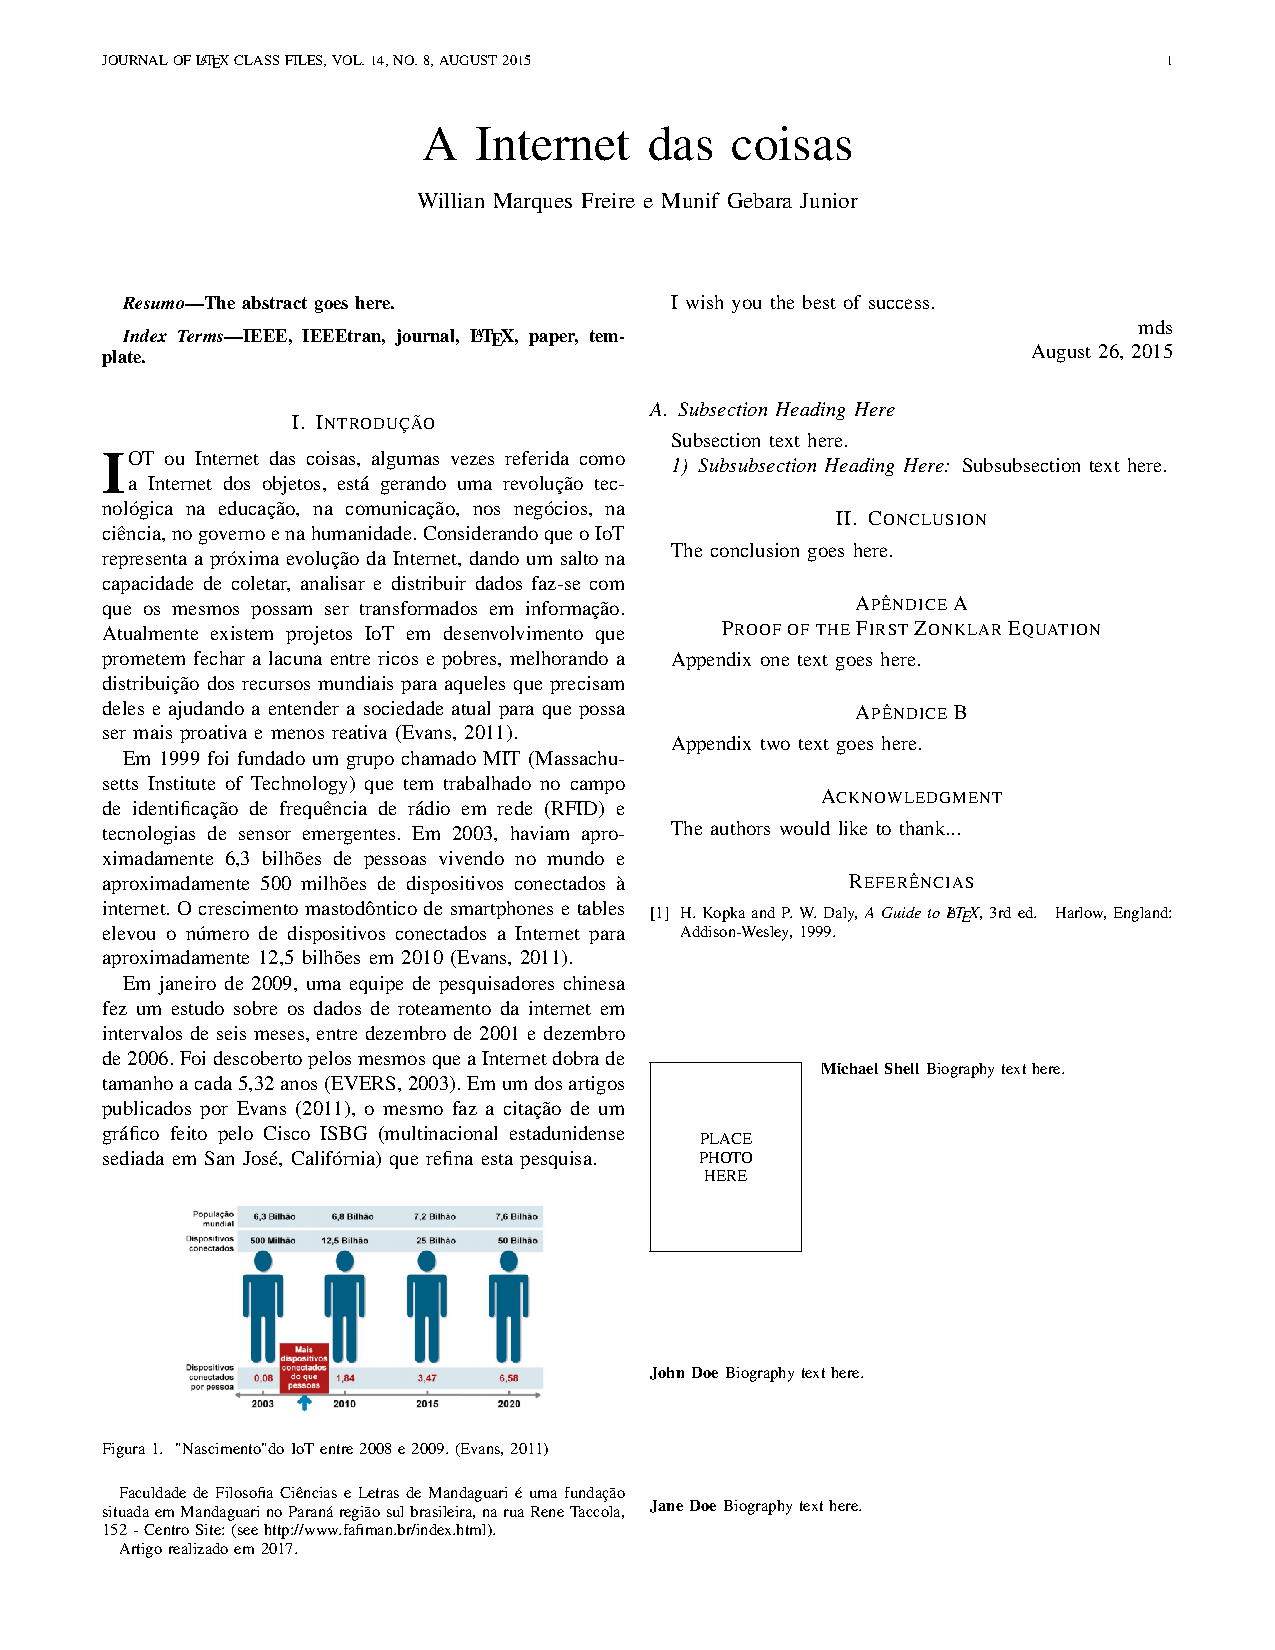
\includepdf[pages=-, offset=75 -75]{artigos/artigo1/bare_jrnl.pdf}
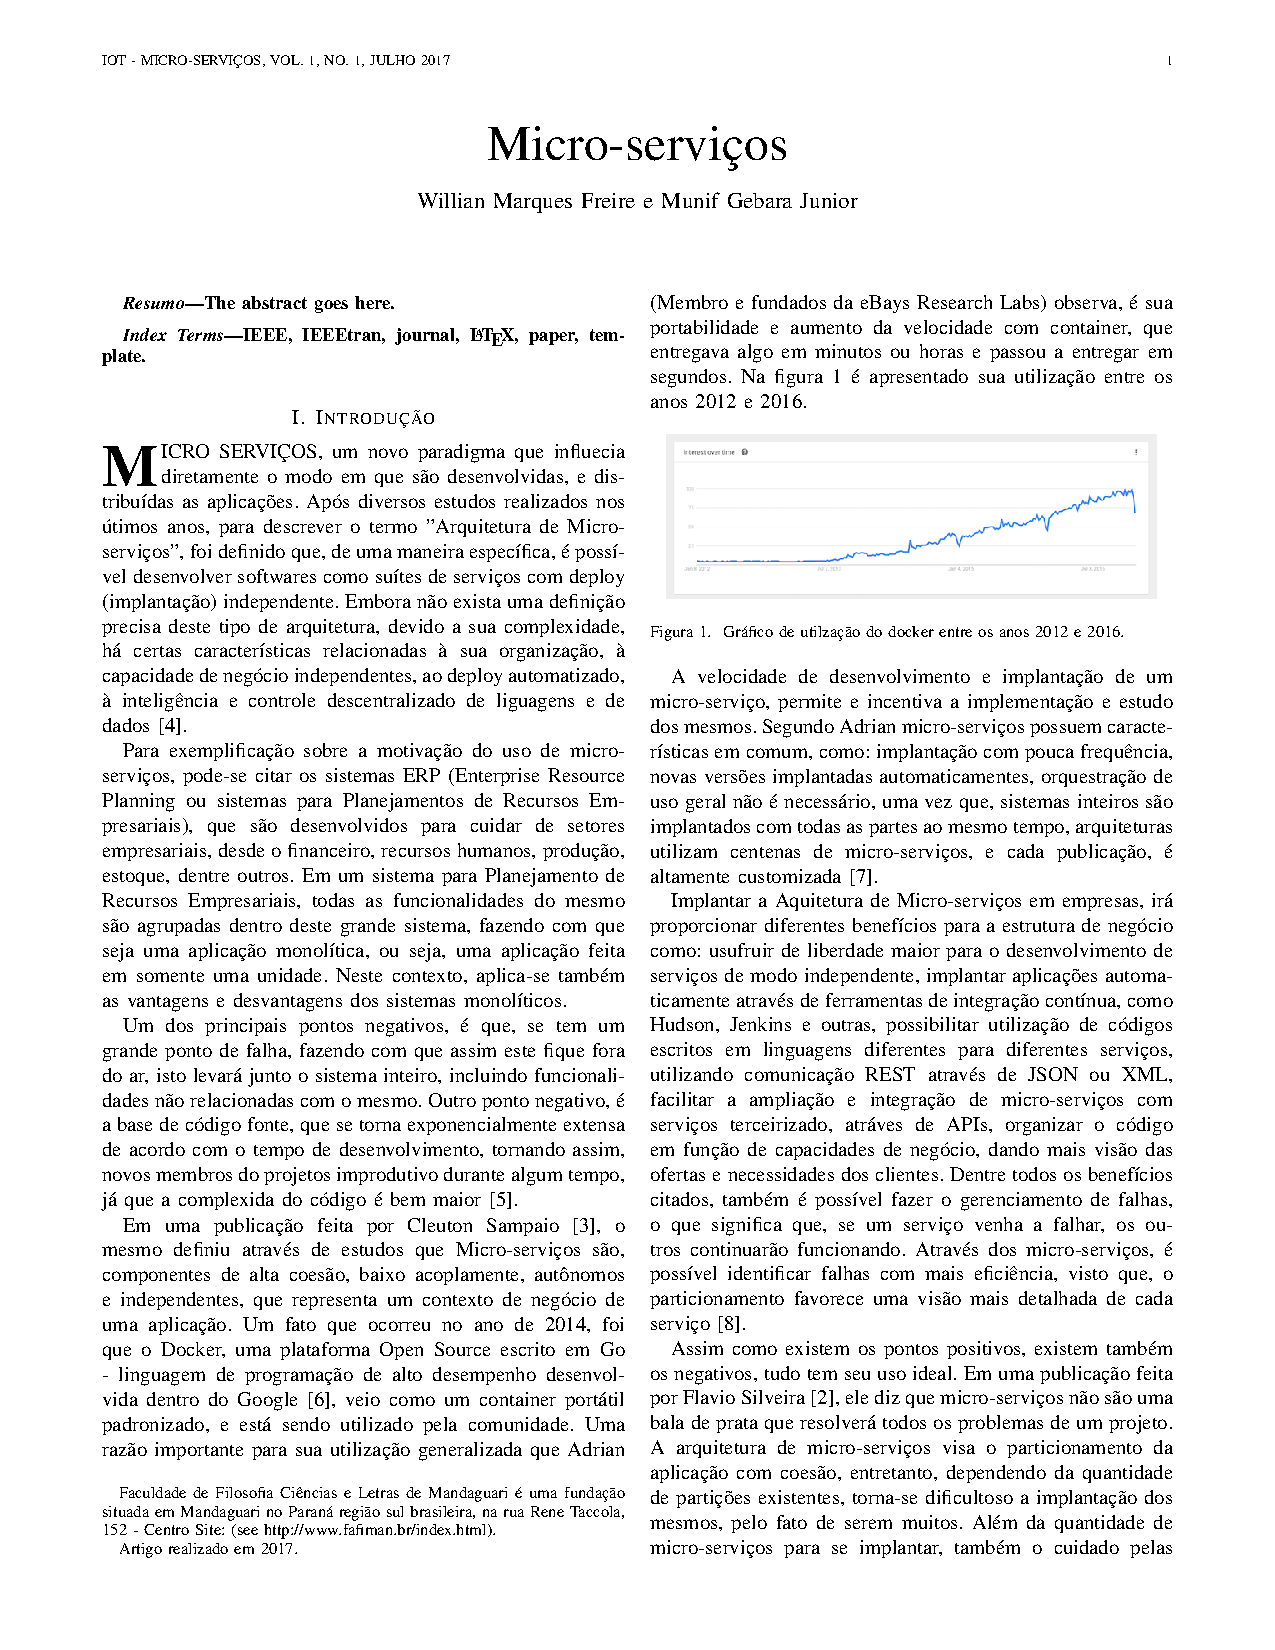
\includepdf[pages=-, offset=75 -75]{artigos/artigo2/bare_jrnl.pdf}
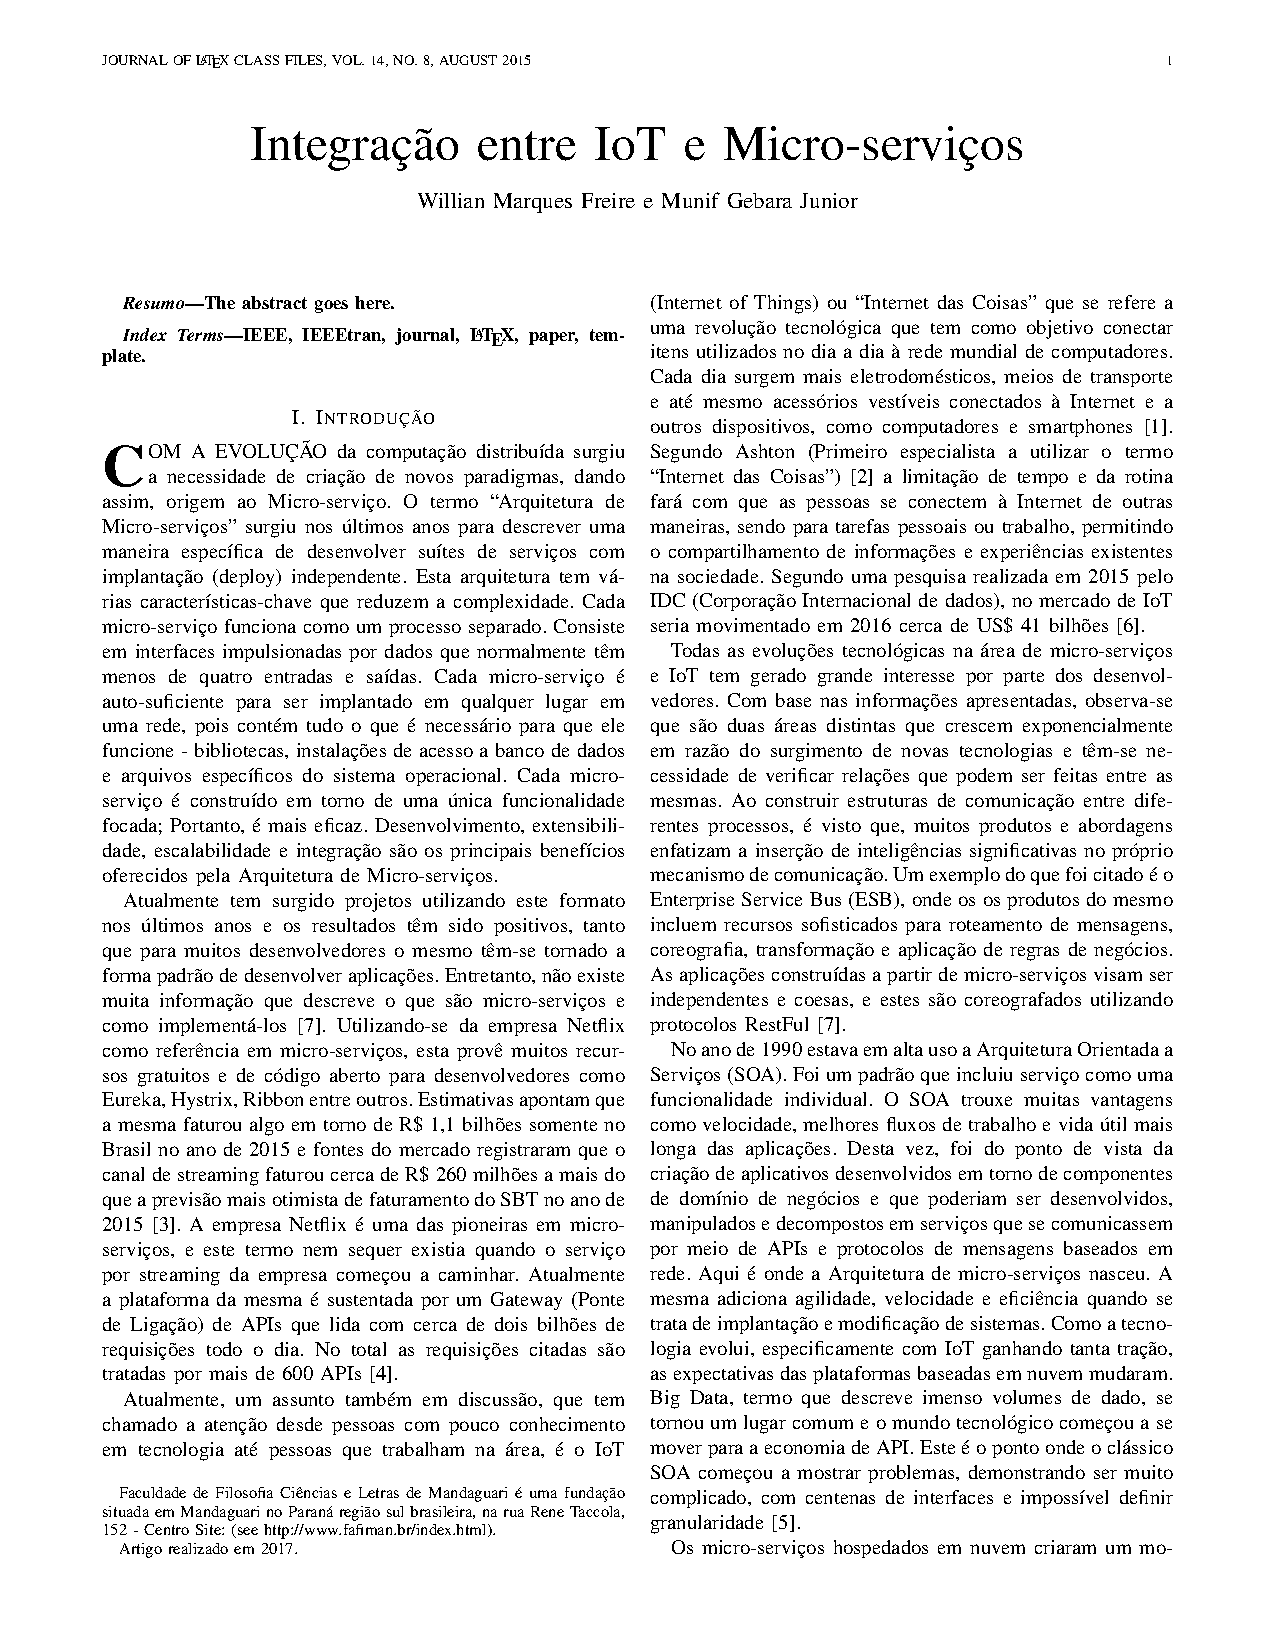
\includepdf[pages=-, offset=75 -75]{artigos/artigo3/bare_jrnl.pdf}

\setlength{\voffset}{0cm}
\setlength{\hoffset}{0cm}


\section{APRESENTAÇÃO E ANÁLISE DOS RESULTADOS}
Toda pesquisa deve apresentar uma análise sobre a investigação que foi realizada através da metodologia que foi aplicada. Nesta sessão é interessante inserir tabelas, gráficos, imagens que mostrem os resultados, análise de dados coletados, etc.

É interessante que nessa sessão o autor compare os seus resultados com os resultados de outros trabalhos existentes. Essa comparação aumenta a qualidade do trabalho e demonstra a relevância do mesmo. 

Nesta sessão o autor pode/deve incluir as contribuições científicas desenvolvidas tais como artigos, patentes, livros e outras contibuições que foram publicadas ou estão em fase de publicação e que são parte do trabalho.
\section{CONCLUSÕES E TRABALHOS FUTUROS}
A conclusão deve conter os principais aspectos e contribuições de forma a finalizar o trabalho apresentado. Deve-se apresentar o que era esperado do trabalho através dos objetivos inseridos inicialmente e mostrar o que foi conseguido. 

	Não deve-se inserir um novo assunto na conclusão. Aqui o autor apresentará as próprias impressões sobre o trabalho efetuado. 
    
É importante também que sejam identificadas limitações e problemas que surgiram durante o desenvolvimento do trabalho e quais as consequências do mesmo.

Os trabalhos futuros devem conter oportunidades de expansão do trabalho apresentado, bem como, novos projetos que puderam ser vislumbrados a partir do desenvolvimento do trabalho
%%%%%%%%%%%%%%%%%%%%%%%%%%%%% Referências %%%%%%%%%%%%%%%%%%%%%%%%%%%%%
\renewcommand{\refname}{\centering REFERÊNCIAS} %Centraliza nome Referencias%
\addcontentsline{toc}{section}{REFERÊNCIAS} %adiciona referencias ao sumario

\nocite{*}
\bibliographystyle{plain}
\bibliography{references}

%%%%%%%%%%%%%%%%%%%%%%%%%%%%%%%%%%%%%%%%%%%%%%%%%%%%%%%%%%%%%%%%%%%%%%%

%%%%%%%%%%%%%%%%%%%%%%%%%%%%% ANEXO %%%%%%%%%%%%%%%%%%%%%%%%%%%%%
\section*{\centering{A – ANEXOS E APÊNDICES 1}}
\addcontentsline{toc}{section}{A - ANEXOS E APÊNDICES 1}

Anexos e apêndices são materiais adicionais, utilizados para complementar o texto, acrescentados ao final do trabalho, com a finalidade de esclarecimento ou de comprovação.

Apêndices são elaborados pelo autor e visam complementar uma argumentação. Os Anexos não são elaborados diretamente pelo autor e servem de fundamentação teórica, comprovação e ilustração (ex. mapas, leis, estatutos entre outros). Os apêndices devem aparecer antes dos anexos.



\end{document}